\documentclass[11pt]{article}

% ====================================================
% PACKAGES
% ====================================================
\usepackage[margin=1in, headheight=13.6pt]{geometry}
\usepackage[T1]{fontenc}
\usepackage{lmodern}
\usepackage{microtype}
\usepackage{setspace}
\usepackage{tcolorbox}
\usepackage{amsmath, amssymb, mathtools}
\usepackage{siunitx}
\usepackage{bm}

\usepackage{graphicx}
\usepackage{float}
\usepackage{subcaption}

\usepackage{enumitem}
\usepackage{booktabs}
\usepackage{longtable}
\usepackage{array}
\usepackage{multirow}

\usepackage{xcolor}
\usepackage{hyperref}

\usepackage{fancyhdr}
\usepackage{lastpage}

\usepackage{indentfirst}
\usepackage[justification=centering]{caption}
\usepackage{pdfpages}
\usepackage{listings}

\lstdefinestyle{pystyle}{
    language=Python,
    basicstyle=\ttfamily\small,
    keywordstyle=\color{blue!60!black}\bfseries,
    commentstyle=\color{green!40!black}\itshape,
    stringstyle=\color{orange!70!black},
    numbers=left,
    numberstyle=\tiny\color{gray},
    numbersep=6pt,
    breaklines=true,
    breakatwhitespace=false,
    showstringspaces=false,
    frame=single,
    rulecolor=\color{gray!50},
    tabsize=4
}
\lstset{style=pystyle}

\pagestyle{fancy}
\fancyhf{}
\lhead{\Assignment\ |\ \course}
\rhead{\Name\ |\ \today}
\cfoot{Page \thepage\ of~\pageref{LastPage}}

\hypersetup{
    colorlinks,
    linkcolor={red!50!black},
    citecolor={blue!50!black},
    urlcolor={blue!80!black}
}

\newcommand{\Name}{Arael Anaya}
\newcommand{\Assignment}{Homework 2}
\newcommand{\course}{Robot Mechanics}

% Boxed final-answer environment
\newtcolorbox{result}{
    colback=blue!3!white,
    colframe=blue!40!black,
    boxrule=0.6pt,
    arc=2pt,
    left=6pt, right=6pt, top=4pt, bottom=4pt
}

% Boxed problem-statement environment
\newtcolorbox{statement}{
    colback=gray!5!white,
    colframe=gray!50!black,
    boxrule=0.4pt,
    arc=2pt,
    left=6pt, right=6pt, top=4pt, bottom=4pt
}

% Visible placeholder for work not yet added
\newcommand{\workplaceholder}{%
    \par\vspace{4pt}\noindent\textcolor{gray!60}{\itshape [Work not yet added: paste solution here]}\par\vspace{4pt}%
}

% Boxed correction-note environment (flags a fix made to the original hand calc)
\newtcolorbox{fixnote}{
    colback=orange!5!white,
    colframe=orange!55!black,
    boxrule=0.5pt,
    arc=2pt,
    left=6pt, right=6pt, top=4pt, bottom=4pt,
    fontupper=\small
}

% Notation macros (matching course conventions)
\newcommand{\T}{\bm{T}}
\newcommand{\R}{\bm{R}}
\newcommand{\dvec}{\bm{d}}
\newcommand{\framen}[1]{\{#1\}}
\newcommand{\khat}{\widehat{\bm{k}}}
\newcommand{\wvec}{\bm{\omega}}
\newcommand{\Rotx}{\operatorname{Rot}_x}
\newcommand{\Roty}{\operatorname{Rot}_y}
\newcommand{\Rotz}{\operatorname{Rot}_z}
\newcommand{\atantwo}{\operatorname{atan2}}
\newcommand{\skewx}[1]{\left[#1\right]_{\times}}

\begin{document}

% ====================================================
% APPENDIX A: PYTHON CODE
% ====================================================
\newpage
\section*{Appendix A: Python Code}

\subsection*{Problem 1: Gimbal Degeneracy Sketch}
\lstinputlisting[caption={Problem 1.py: generates the intermediate-rotation sketch in Fig.~1.}]{"../Code/Problem 1.py"}

\newpage
\subsection*{Problem 2: ZYZ Angles, Angle--Axis, and Quaternion}
\lstinputlisting[caption={Problem 2.py: evaluates the ZYZ angles, angle-axis pair, and quaternion for Problem 2.}]{"../Code/Problem 2.py"}

\newpage
\subsection*{Problem 3: Quaternion to Rotation Matrix and Angle--Axis}
\lstinputlisting[caption={Problem 3.py: converts each quaternion in Problem 3 to a rotation matrix and angle-axis pair.}]{"../Code/Problem 3.py"}

% ====================================================
% APPENDIX B: HAND CALCULATIONS
% ====================================================
\newpage
\section*{Appendix B: Hand Calculations}

\begin{fixnote}
\textbf{Corrections made when typing up the hand calcs below:}
\begin{enumerate}[leftmargin=1.2em, itemsep=4pt]
    \item \textbf{Problem 1(b), page 1:} the boxed yaw formula was written as $\phi = \atantwo\!\left(\frac{r_{21}}{c\theta_{\pm}},\ \frac{r_{12}}{c\theta_{\pm}}\right)$, but $r_{12}$ doesn't show up in the $\phi$ equation. The correct value comes from the first column, $r_{21} = s\phi c\theta$ and $r_{11} = c\phi c\theta$ (the same terms $c\theta = \sqrt{r_{11}^{2}+r_{21}^{2}}$ above it is built from). 
    \item \textbf{Problem 3(d), page 6:} the $(1,2)$ entry of the rotation matrix was written as $-0.639$. Evaluating $2(q_{1}q_{2}-q_{0}q_{3}) = 2\big((0.5928)(0.08311)-(0.5332)(0.5978)\big)$ gives $-0.539$, matching the neighbouring entries ($0.271$, $0.797$, $0.736$, $-0.418$, $-0.533$, $0.620$, $0.732$, $0.283$) and the boxed axis $\khat = [0.701\ 0.098\ 0.707]^{T}$ exactly.
\end{enumerate}
\end{fixnote}

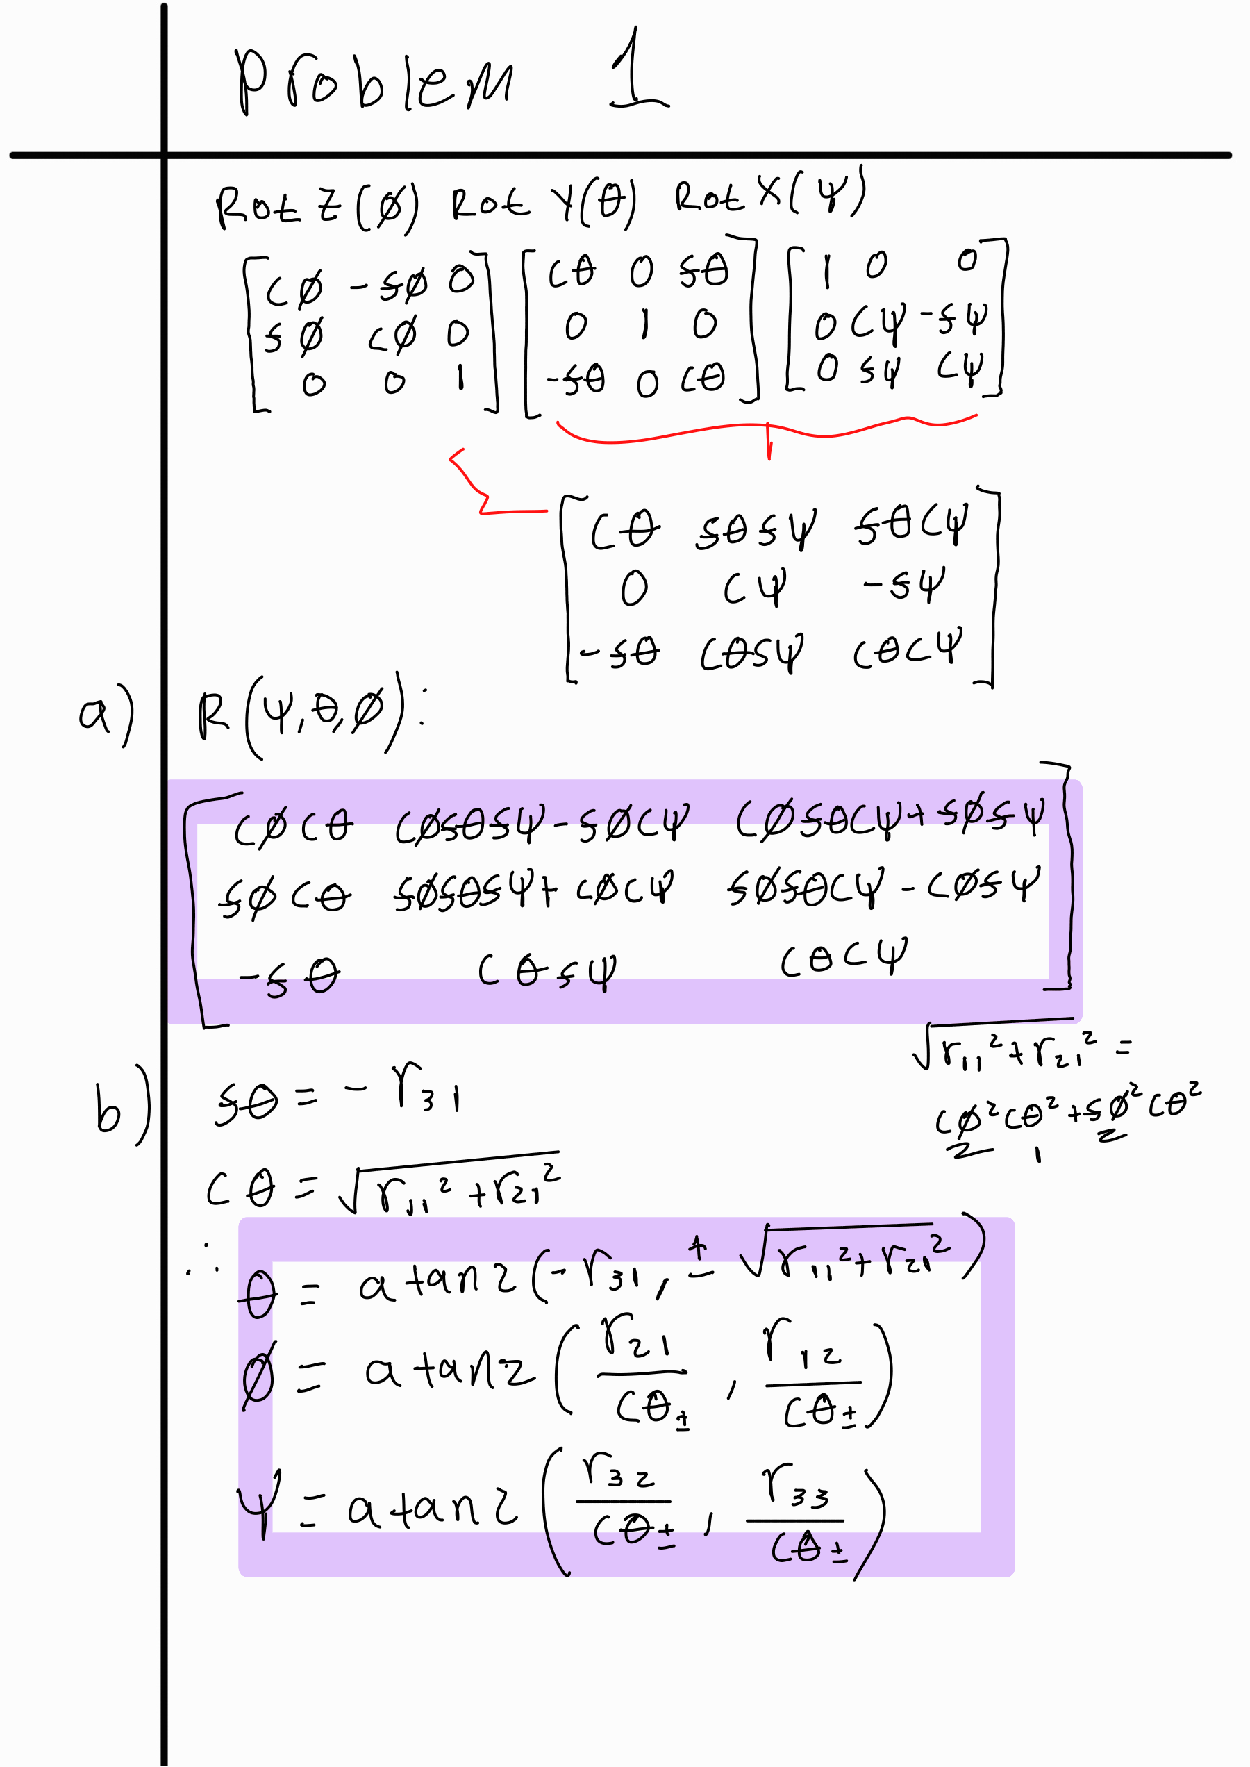
\includepdf[pages=-, pagecommand={\thispagestyle{plain}}, scale=0.9]{../Homework_2_hand_calcs.pdf}

\end{document}
